\section{Results}
\label{sec:results}

\begin{figure*}[t]
  \centering
  \begin{subfigure}[t]{0.245\textwidth}
    \centering
    \captionsetup{width=0.95\textwidth}
    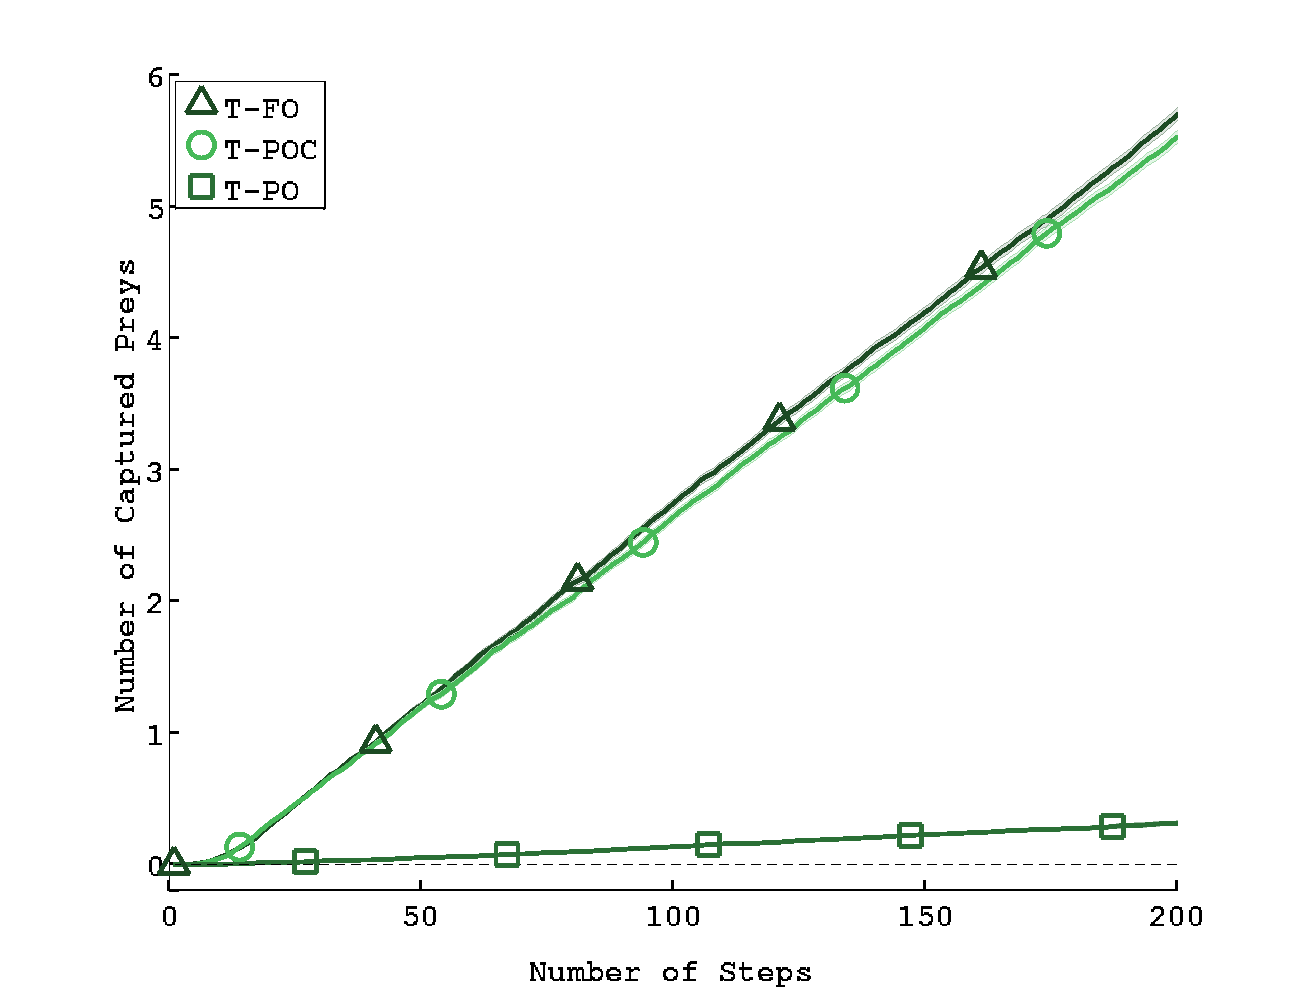
\includegraphics[trim=2.6cm 0.4cm 2.7cm 1.8cm, clip=true, width=\figwidth\textwidth]{plots/with_noise/teamComparaison.png}
    \caption{Comparison of teams with full observability (\emph{T-FO}), partial observability without (\emph{T-PO}) and with (\emph{T-POC}) communication. The use of communication in the partial observability case allows recovering similar performances than with full observability. %Only cases where no predators can see the prey reduce performances.
}
    \label{fig:cmpteam}
  \end{subfigure}
  \begin{subfigure}[t]{0.245\textwidth}
    \centering
    \captionsetup{width=0.9\textwidth}
    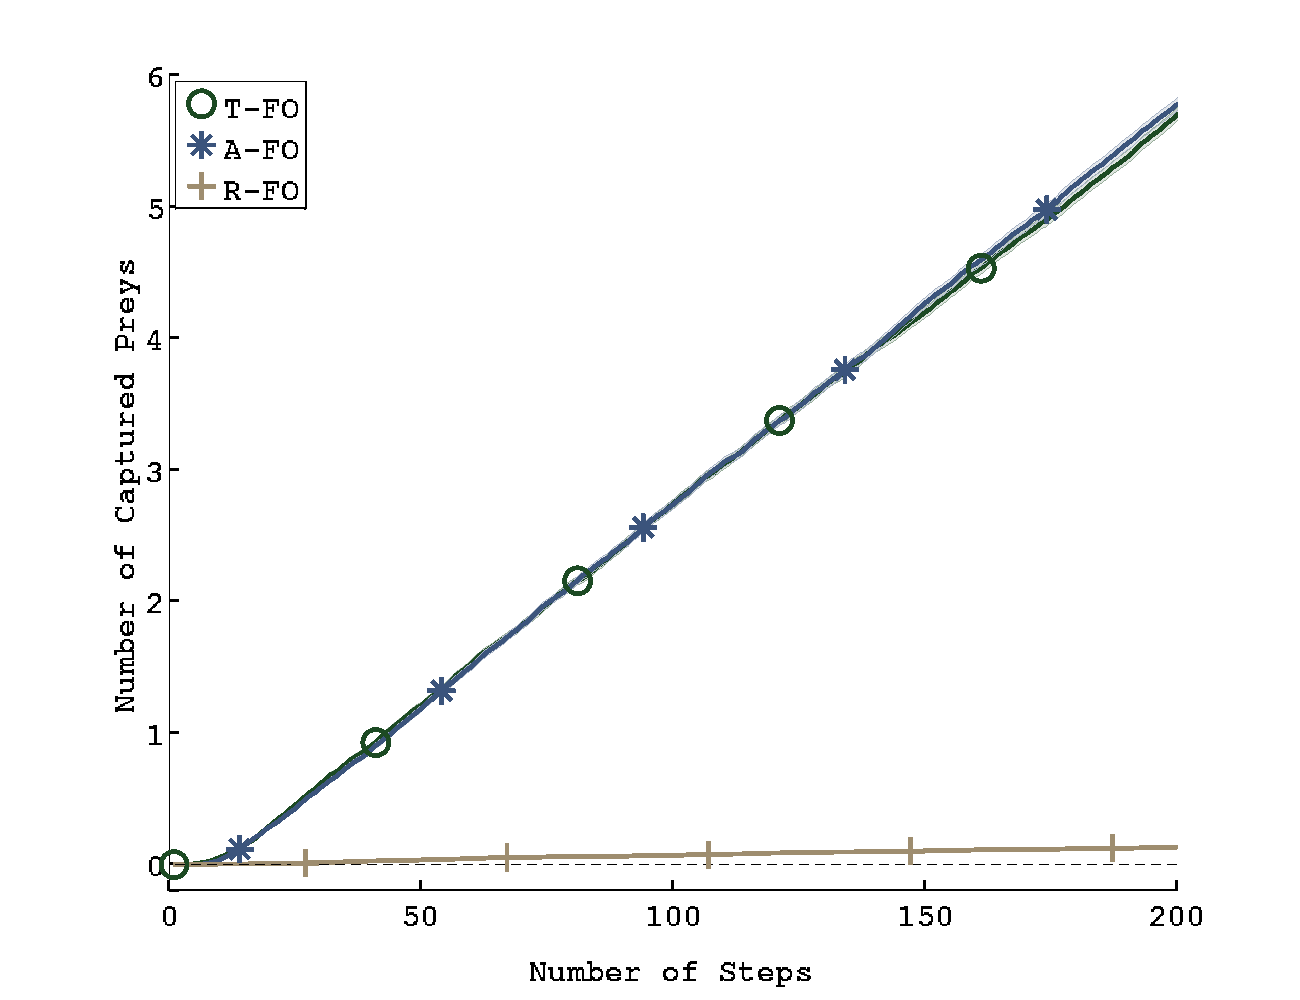
\includegraphics[trim=2.6cm 0.4cm 2.7cm 1.8cm, clip=true, width=\figwidth\textwidth]{plots/with_noise/fullObs.png}
    \caption{Comparison of default team (\emph{T-FO}), ad hoc team (\emph{A-FO}), or a team including a predator with random policy (\emph{R-FO}). All predators have full observability. The inclusion of our ad hoc agent does not impact the performance.}
    \label{fig:fullobs}
  \end{subfigure}
  \begin{subfigure}[t]{0.245\textwidth}
    \centering
    \captionsetup{width=1.15\textwidth}
    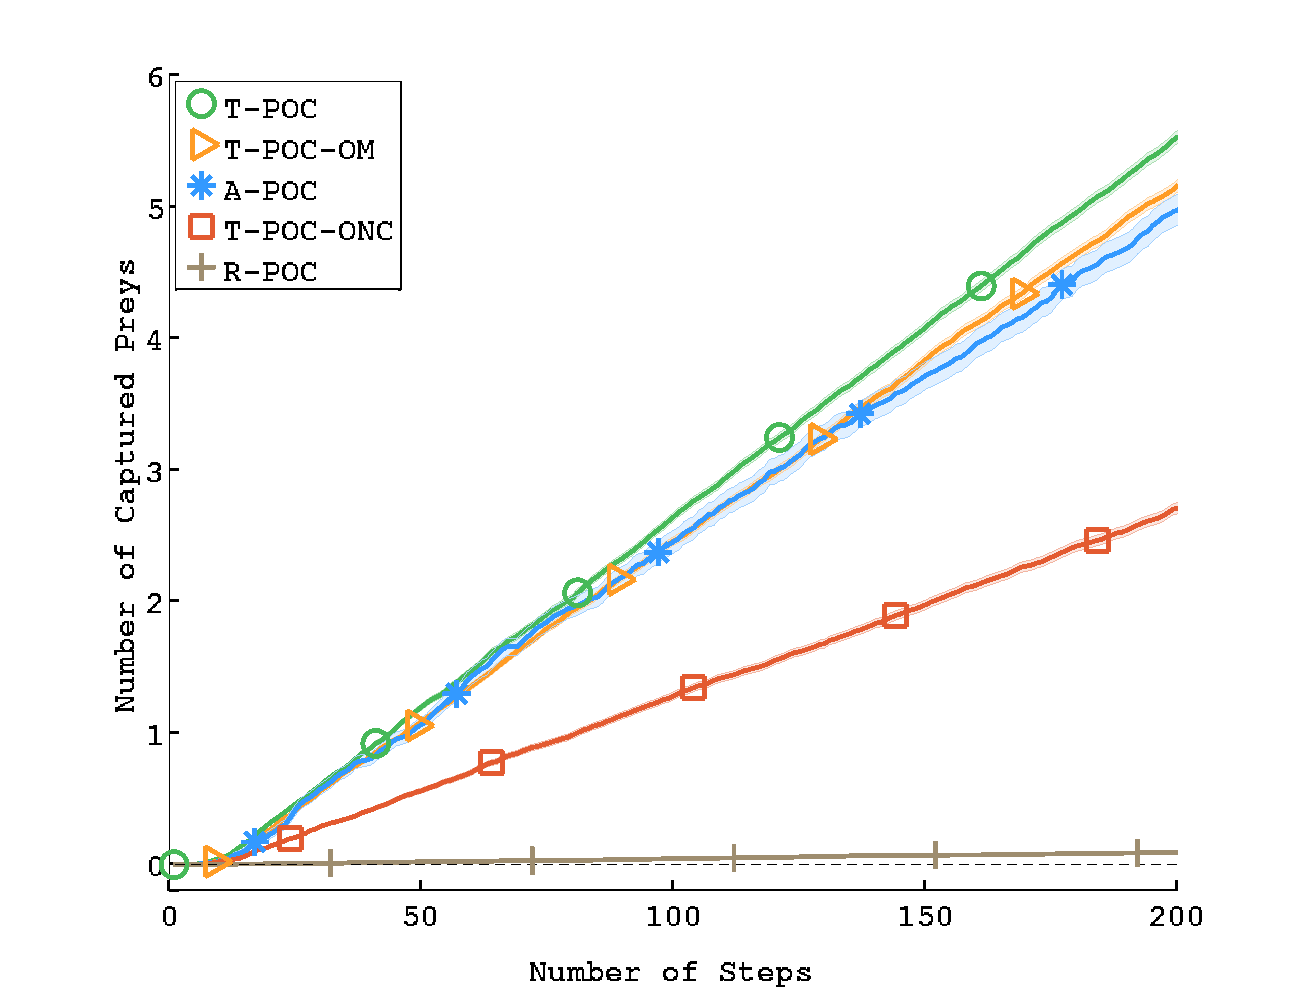
\includegraphics[trim=2.6cm 0.4cm 2.7cm 1.8cm, clip=true,width=\figwidth\textwidth]{plots/with_noise/partialObsCom.png}
    \caption{Comparison of default team (\emph{T-POC}), ad hoc team (\emph{A-POC}), or a team with one muted (\emph{T-POC-OM}) or one non-communicanting (\emph{T-POC-ONC}) predator. All predators have partial observability. The ad hoc agent does not communicate. The inclusion of our ad hoc agent does not impact the performances compared to \emph{T-POC-OM}.}
    \label{fig:partialobscom}
  \end{subfigure}
  \begin{subfigure}[t]{0.245\textwidth}
    \centering
    \captionsetup{width=0.62\textwidth}
    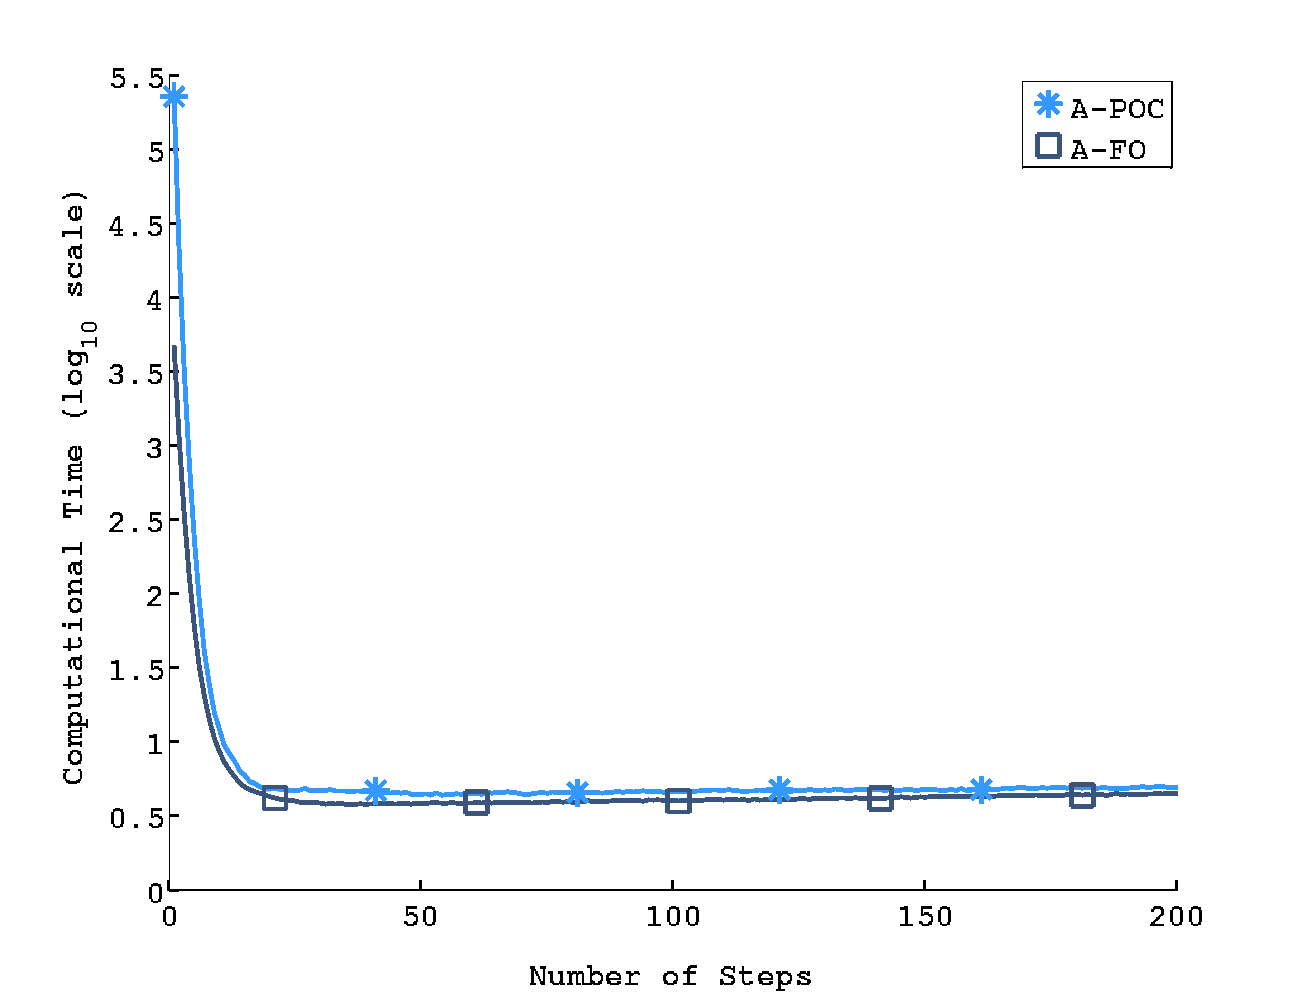
\includegraphics[trim=1.5cm 0.3cm 2.7cm 1.8cm, clip=true,width=\figwidth\textwidth]{plots/with_noise/computationalTime.png}
    \caption{After 20 steps, most hypotheses are discarded and the updates become faster. \emph{A-FO} (respectively \emph{A-POC}) disambiguates between 100 (respectively 1000) hypotheses.}
    \label{fig:comptime}
  \end{subfigure}
  \caption{(a) (b) (c) Average number of preys captured through steps for different conditions. (d) Computational time per step (log scale) for the ad hoc agent. All results include 20 percent of noise in actions and communications.\vspace{-0.3cm}}
  \label{fig:results}
\end{figure*}

We now present several experiments to evaluate how an ad hoc agent can join a team for which it does not know the specific task, its role, and the communication signals being used. We will compare several teams: a pre-formed team (\emph{T}), a team including the ad hoc agent (\emph{A}), and a few baseline described next. We consider several different conditions that affect the team efficiency and the difficulty for the ad hoc agent to join the team: full observability (\emph{FO}) and partial observability without (\emph{PO}) and with (\emph{POC}) communication. We present results with 20 percent of noise in the action and communication as described in Section~\ref{sec:domain}.

For each experiment run we randomly create a domain set $D$, comprised of a set of 10 task hypotheses, 10 team configurations, and 10 communication protocols; resulting in 1000 domains. Among this set, one configuration was selected for the team but was unknown to the ad hoc agent. All the figures presented next display the mean and standard error of the variable considered. Standard errors are shown has a shaded area, but, given the high number of samples (1000 runs using the same random seed for all conditions), it is barely visible. Statistical results presented are two-sample t-test to determine if the average final scores of teams are equal.

The code to reproduce these results is available online at \url{https://github.com/jgrizou/adhoc_com}.

A team of agents is evaluated by its total reward accumulated in 200 steps, i.e. the number of time the prey was captured. After each capture of the prey, the predators and the prey position are randomly reassigned. The capture state, the team configuration, and the communication protocol do not change during the 200 steps.

%\subsubsection*{Implementation details}

%For each run, each condition was initialized with the same random seed, meaning that the initial position, role, capture state, and communication protocol was the same for all experimental conditions of the same run. After each capture, the random seed was incremented by one, the random generator was reseted with this new seed, and the positions of the agent were randomly reassigned. That way, we ensure that for each condition the successive reinitialization of positions are similar. This is important for comparing the results in a meaningful way because of the nature of the problem -- starting conditions impact the time needed to capture the prey.

%All agents, including the prey, first select their actions that are then applied in a specific order. The ordering is randomized each step among the predators, the prey action is always applied last. Occupied states are considered as obstacles and cannot be reached. \todo{this can either be removed or moved to the domain section}

\vspace{-0.3cm}
\paragraph{Default Team Performance}

We start by showing how the different conditions affect the behavior of the pre-coordinated team (Figure~\ref{fig:cmpteam}). Partial observability (\emph{T-PO}) dramatically impacts the performance of the team, but it is recovered by the use of communication (\emph{T-POC}). Yet, \emph{T-POC} does not catch up with \emph{T-FO} (the null hypothesis is rejected with {\small$p=0.014$}) because in some configurations none of the agents can see the prey. %As expected adding 20\% of noise in the movements and communication decreases the performance of the teams, capturing on average 5 times the prey in 200 steps instead of 15 when no noise is applied. Results can be seen in Fig.~\ref{fig:cmpteam}.

% \begin{figure}[htbp!]
%   \centering
%   \begin{subfigure}[b]{0.49\columnwidth}
%     \centering
%     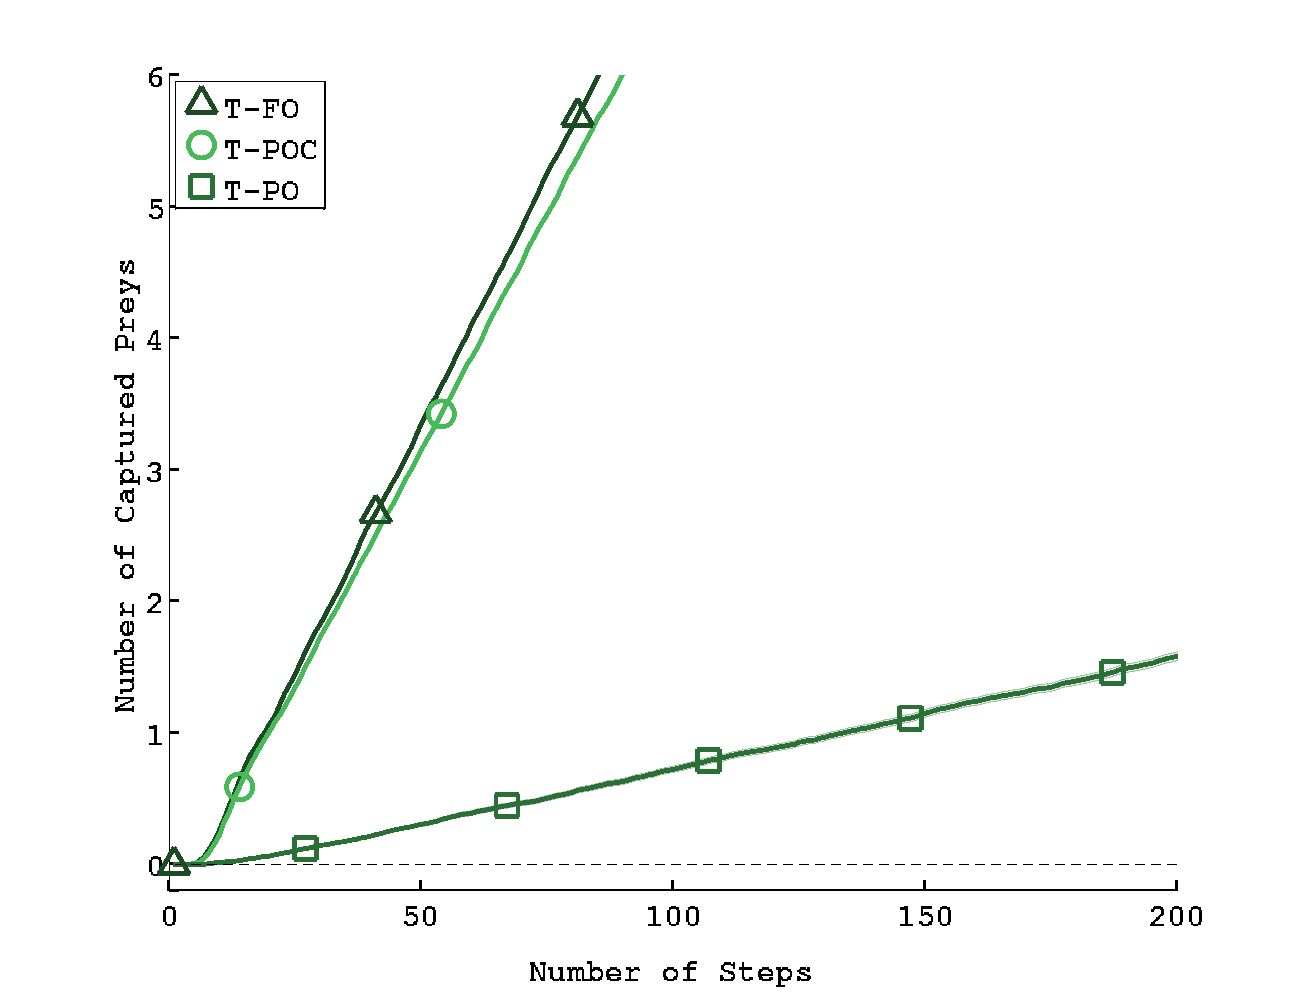
\includegraphics[trim=2.6cm 0.9cm 2.7cm 1.8cm, clip=true, width=\columnwidth]{plots/no_noise/teamComparaison.png}
%     \caption{Without noise}
%     \label{subfig:cmpteamnonoise}
%   \end{subfigure}
%   \begin{subfigure}[b]{0.49\columnwidth}
%     \centering
%     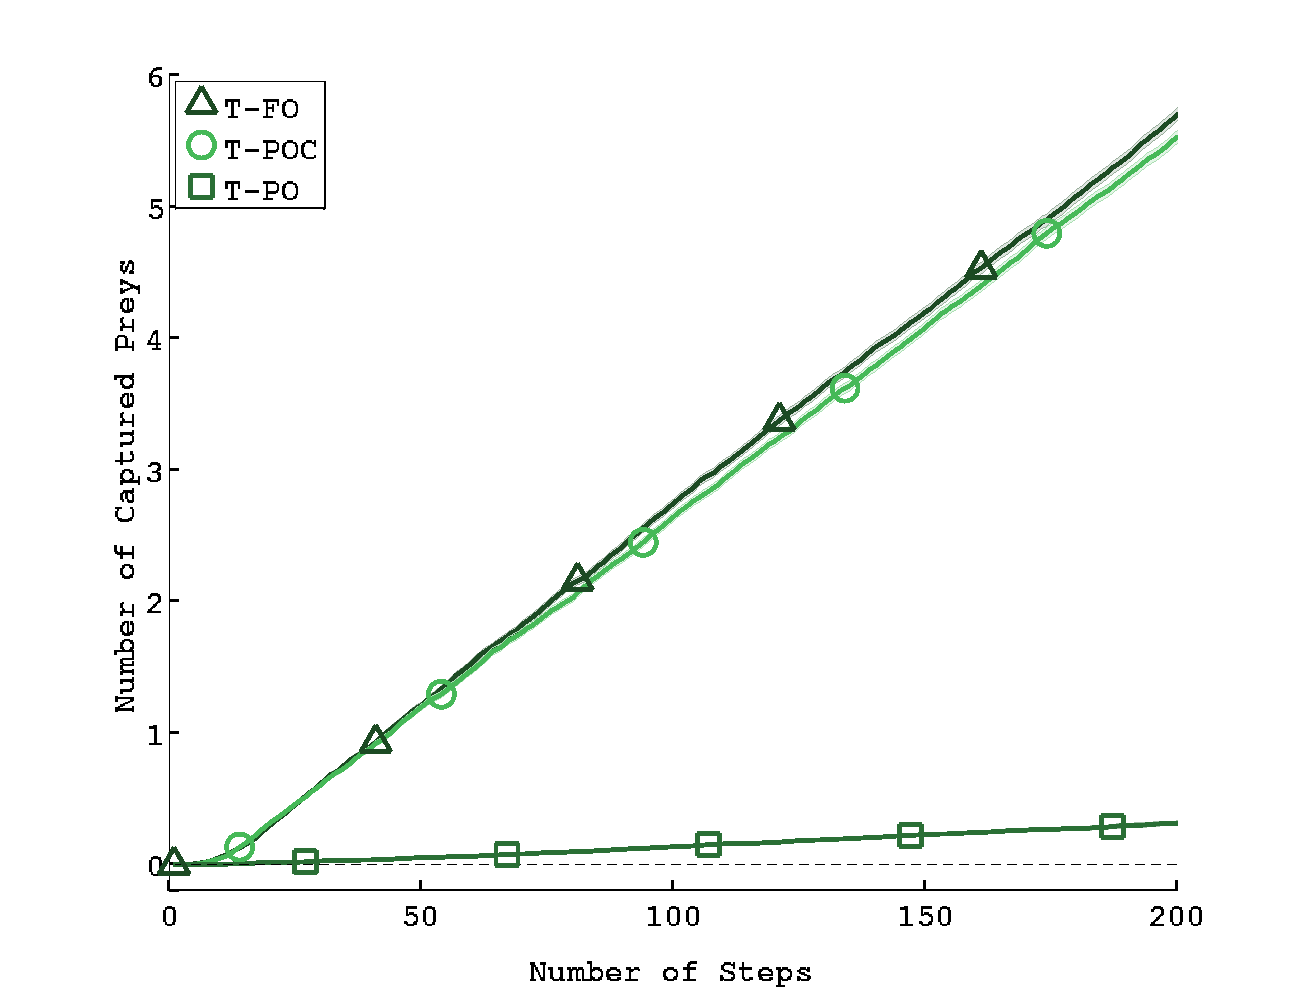
\includegraphics[trim=2.6cm 0.9cm 2.7cm 1.8cm, clip=true, width=\columnwidth]{plots/with_noise/teamComparaison.png}
%     \caption{With 20\% noise}
%     \label{subfig:cmpteamwithnoise}
%   \end{subfigure}
%   \caption{Average number of prey captured through steps, with (right) or without (left) noise. Comparison of teams with full observability (\emph{T-FO}), partial observability without (\emph{T-PO}) and with (\emph{T-POC}) communication. The use of communication in the partial observability allows recovering similar performance than with full observability. Only cases where no predators can see the prey reduce performances.}
%   \label{fig:cmpteam}
% \end{figure}

\vspace{-0.3cm}
\paragraph{Ad Hoc with Full Observability}

We now remove one of the agents from the standard team and replace it with our ad hoc agent (Figure~\ref{fig:fullobs}). In the case of full observability the inclusion of the ad hoc agent has no impact, on average, on the team performance (\emph{T-FO} vs \emph{A-FO} -- the null hypothesis cannot be rejected with {\small$p=0.276$}). It means that the ad hoc agent can correctly identify the correct team configuration without impacting the behavior of the full team. As a point of comparison, we added the performance of a team with one of the agents acting randomly (\emph{R-FO}). Such team almost never captures the prey.

% \begin{figure}[htbp!]
%   \centering
%   \begin{subfigure}[b]{0.49\columnwidth}
%       \centering
%       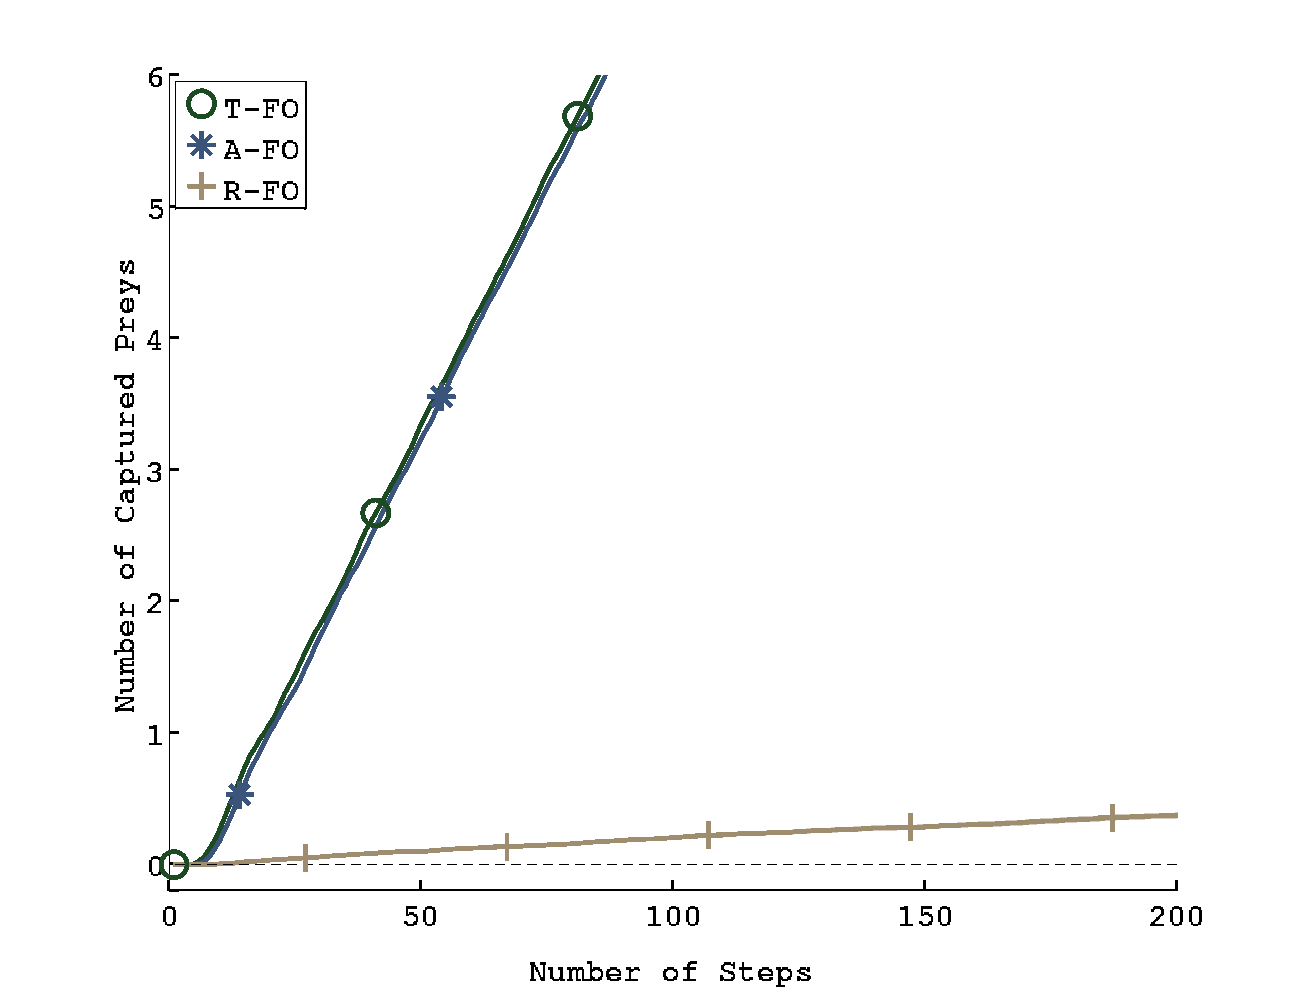
\includegraphics[trim=2.6cm 0.9cm 2.7cm 1.8cm, clip=true,width=\columnwidth]{plots/no_noise/fullObs.png}
%       \caption{Without noise}
%       \label{subfig:fullobsnonoise}
%   \end{subfigure}
%   \begin{subfigure}[b]{0.49\columnwidth}
%     \centering
%     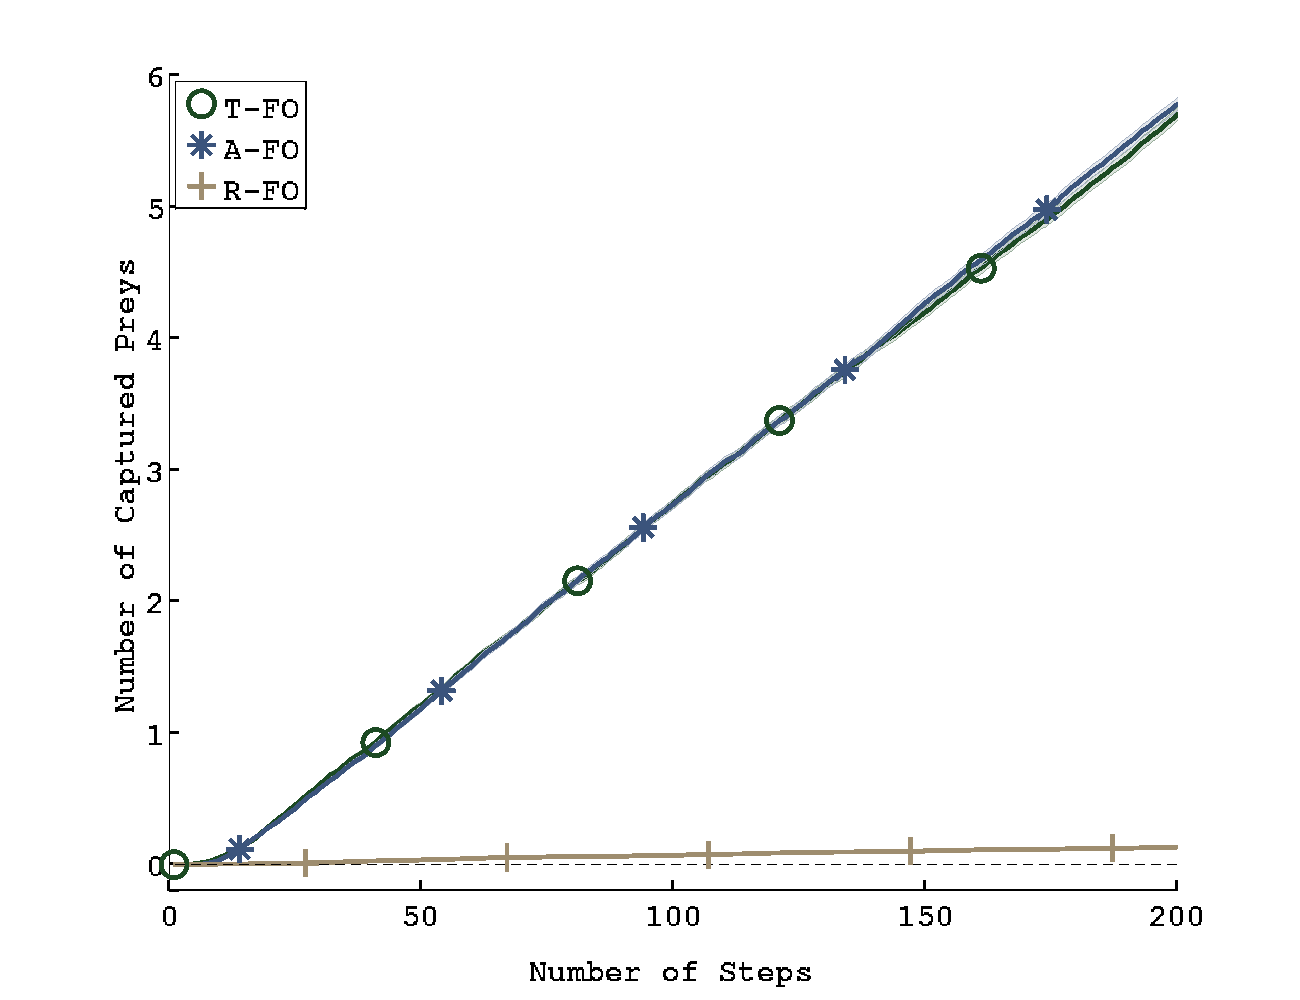
\includegraphics[trim=2.6cm 0.9cm 2.7cm 1.8cm, clip=true,width=\columnwidth]{plots/with_noise/fullObs.png}
%     \caption{With 20\% noise}
%     \label{subfig:fullobswithnoise}
%   \end{subfigure}
%   \caption{Average number of prey captured through steps, with (right) or without (left) noise. Comparison of default team (\emph{T-FO}), ad hoc team (\emph{A-FO}), or a team including a predator with random policy (\emph{R-FO}). All predators have full observability. The inclusion of our ad hoc agent does not impact the performance.}
%   \label{fig:fullobs}
% \end{figure}

\vspace{-0.3cm}
\paragraph{Ad Hoc with Partial Observability}

A more interesting case is when agents act under partial observability. Here the communication has a fundamental role and it will be harder for the ad hoc agent to estimate it besides its required role and the team task. We can see in Figure~\ref{fig:partialobscom} that the ad hoc agent is able to successfully estimate task, role, and communication. In the long term, even in presence of partial observability, the inclusion of the ad hoc agent has a small impact, on average, on the team performance (the null hypothesis is rejected with {\small$p<0.001$}). The gap performance with a pre-formed team could not be reduced further because the ad hoc agent is not able to use communication itself to inform the others. For comparison, we simulated a pre-formed team with one mute agent (\emph{T-POC-OM}) that understand messages but cannot send messages and a pre-formed team with one non communication aware agent (\emph{T-POC-ONC}). Our ad hoc agent performs better than \emph{T-POC-ONC} ({\small$p<0.001$}) and similarly to \emph{T-POC-OM} (the null hypothesis cannot be rejected with {\small$p=0.139$}) despite having 1000 trials, showing that these methods perform similarly.

% , even needing to discriminate between 1000 possible domain hypotheses,

% \begin{figure}[htbp!]
%   \centering
%   \begin{subfigure}[b]{0.49\columnwidth}
%     \centering
%     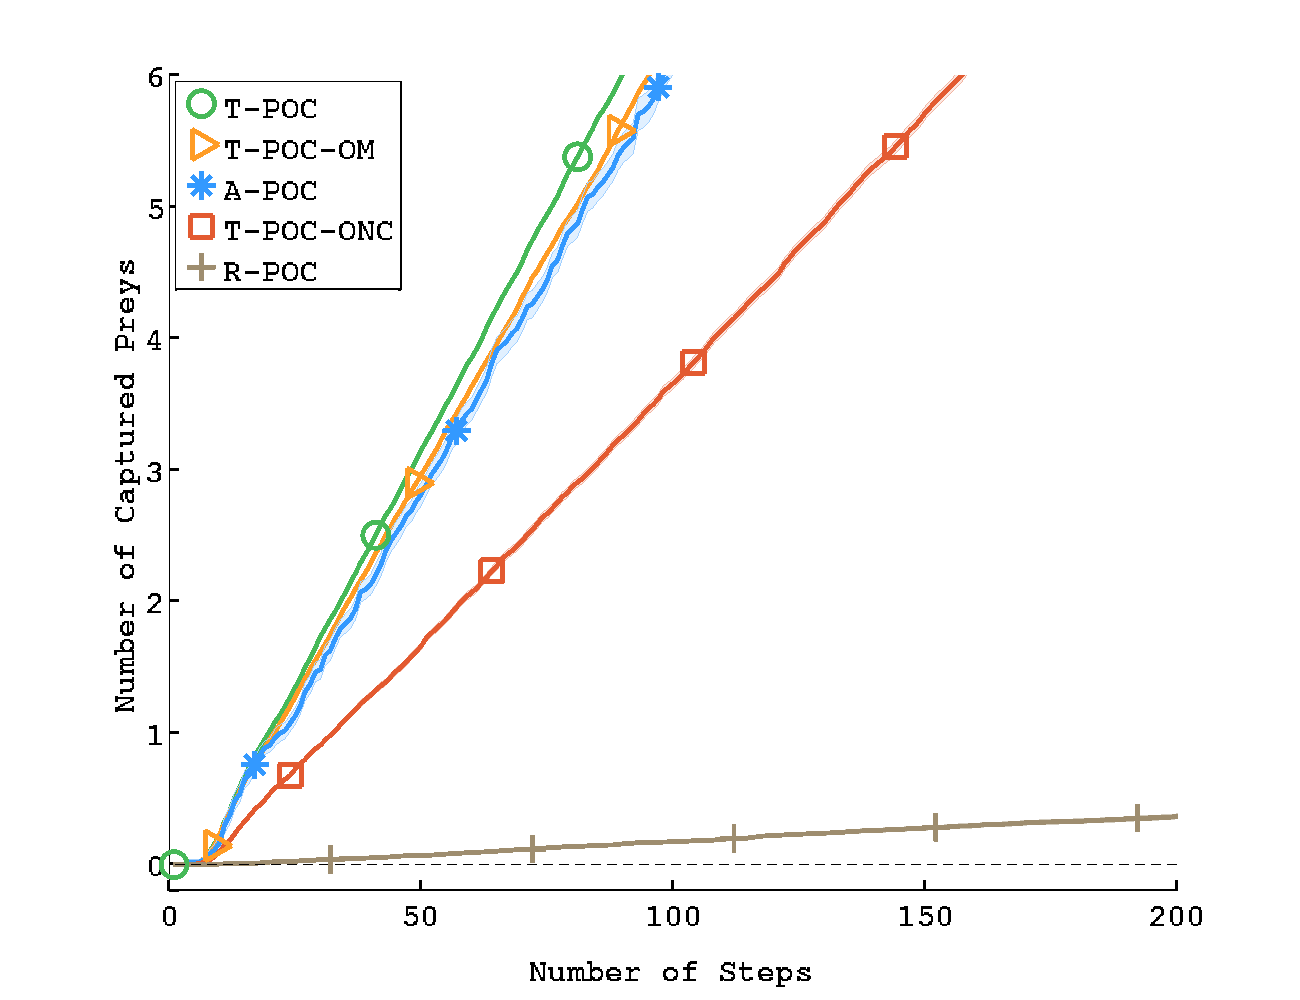
\includegraphics[trim=2.6cm 0.9cm 2.7cm 1.8cm, clip=true,width=\columnwidth]{plots/no_noise/partialObsCom.png}
%     \caption{Without noise}
%     \label{subfig:partialobscomnonoise}
%   \end{subfigure}
%   \begin{subfigure}[b]{0.49\columnwidth}
%     \centering
%     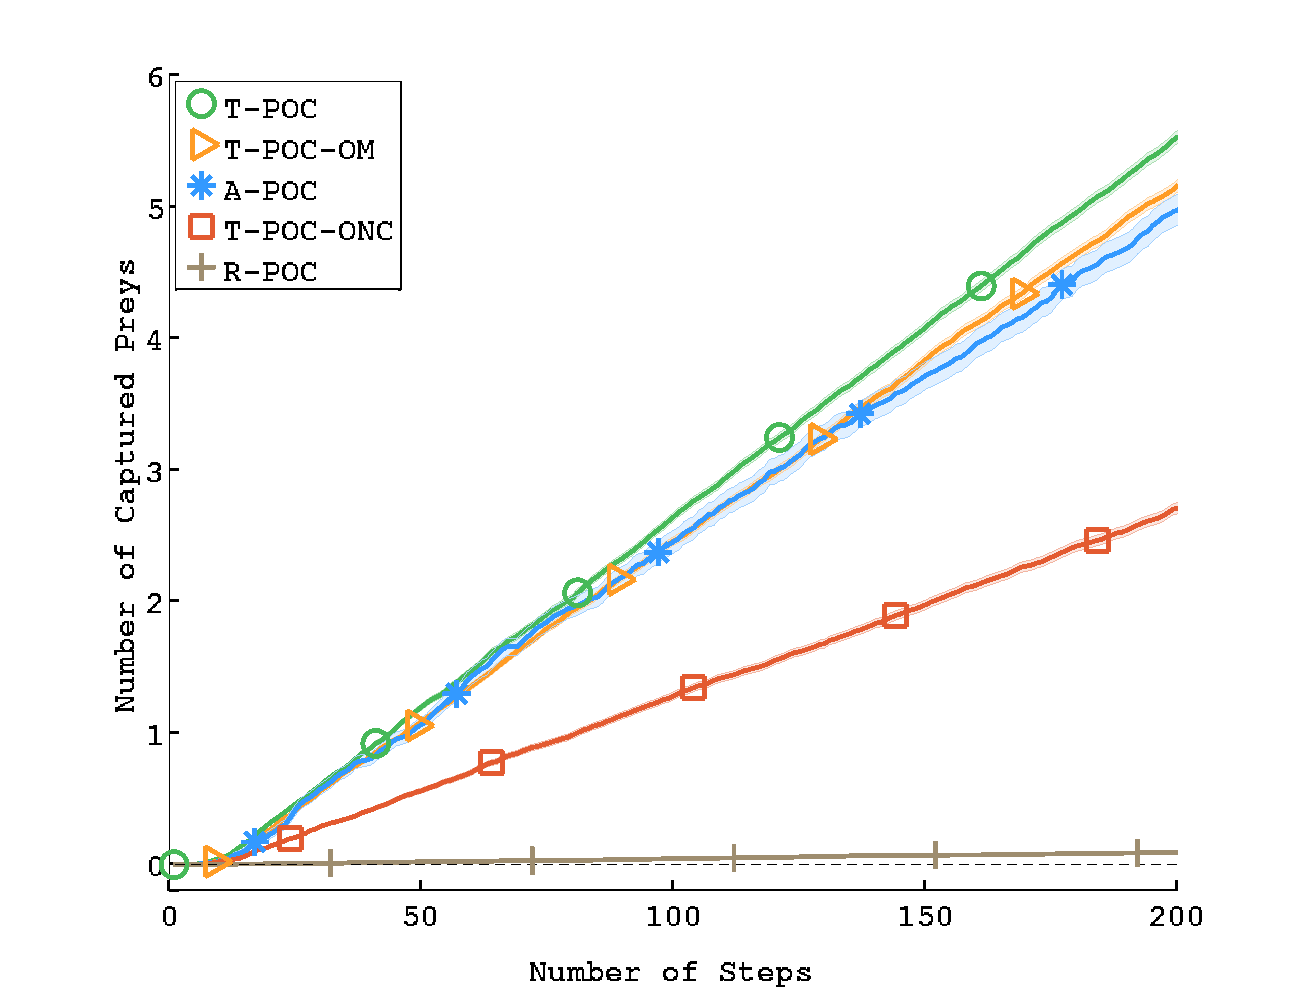
\includegraphics[trim=2.6cm 0.9cm 2.7cm 1.8cm, clip=true,width=\columnwidth]{plots/with_noise/partialObsCom.png}
%     \caption{With 20\% noise}
%     \label{subfig:partialobscomwithnoise}
%   \end{subfigure}
%   \caption{Average number of prey captured through steps, with (right) or without (left) noise. Comparison of default team (\emph{T-POC}), ad hoc team (\emph{A-POC}), or a team including a predator that does not understand communication (\emph{T-POC-ONC}) or that acts randomly (\emph{R-POC}). All predators have partial observability. The ad hoc agent does not communicate. The inclusion of our ad hoc agent does not impact the performance. \todo{include one muted agent}}
%   \label{fig:partialobscom}
% \end{figure}
\vspace{-0.3cm}
\paragraph{Computational Time}

Given the exact inference method we presented, the computational cost is high during the first steps because all hypotheses are still active (Figure~\ref{fig:comptime}). Once an hypothesis is discarded (i.e. reaches a probability of zero), we stop updating its value, reducing the computational cost. The difference between \emph{A-POC} and \emph{A-FO} is due to an increase in the number of hypotheses considered. Indeed, \emph{A-POC} evaluates 1000 hypotheses but \emph{A-FO} evaluates only 100 hypotheses because there is no communication between agents in the full observability case.

% It requires to test for each domain hypotheses the probability of a given outcome given the probability of action of each agent while taking the noise into account. \emph{A-POC} evaluates 1000 hypotheses, \emph{A-FO} evaluates 100 hypotheses. Once an hypothesis is discarded (i.e. reach probability of zero), we stop updating its value reducing the computational cost.

% \begin{figure}[htbp!]
%   \centering
%   \begin{subfigure}[b]{0.49\columnwidth}
%     \centering
%     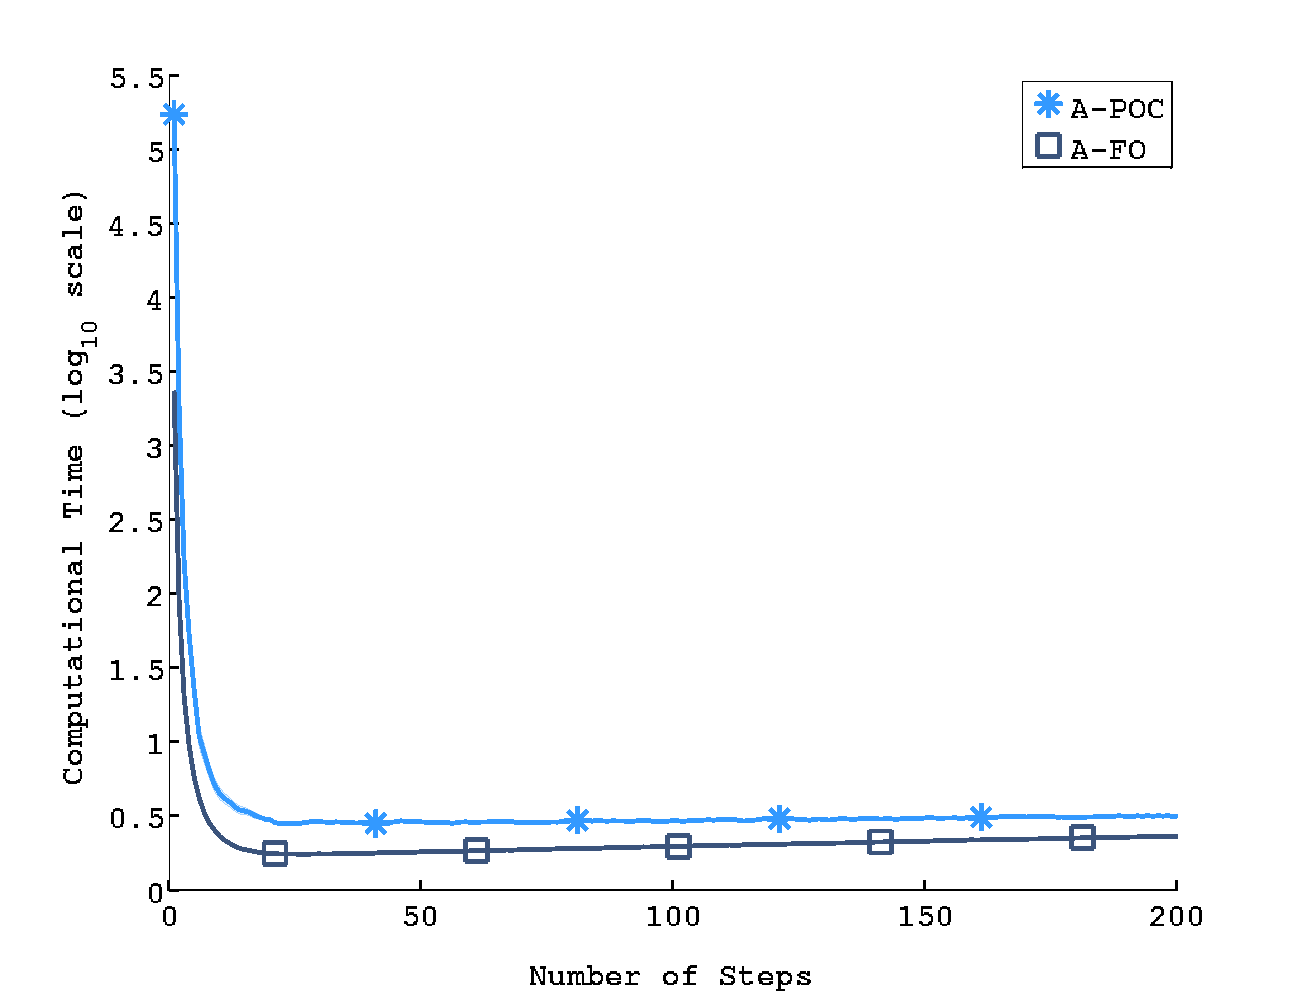
\includegraphics[trim=1.5cm 0cm 2.7cm 1.8cm, clip=true,width=\columnwidth]{plots/no_noise/computationalTime.png}
%     \caption{Without noise}
%     \label{subfig:comptimenonoise}
%   \end{subfigure}
%   \begin{subfigure}[b]{0.49\columnwidth}
%     \centering
%     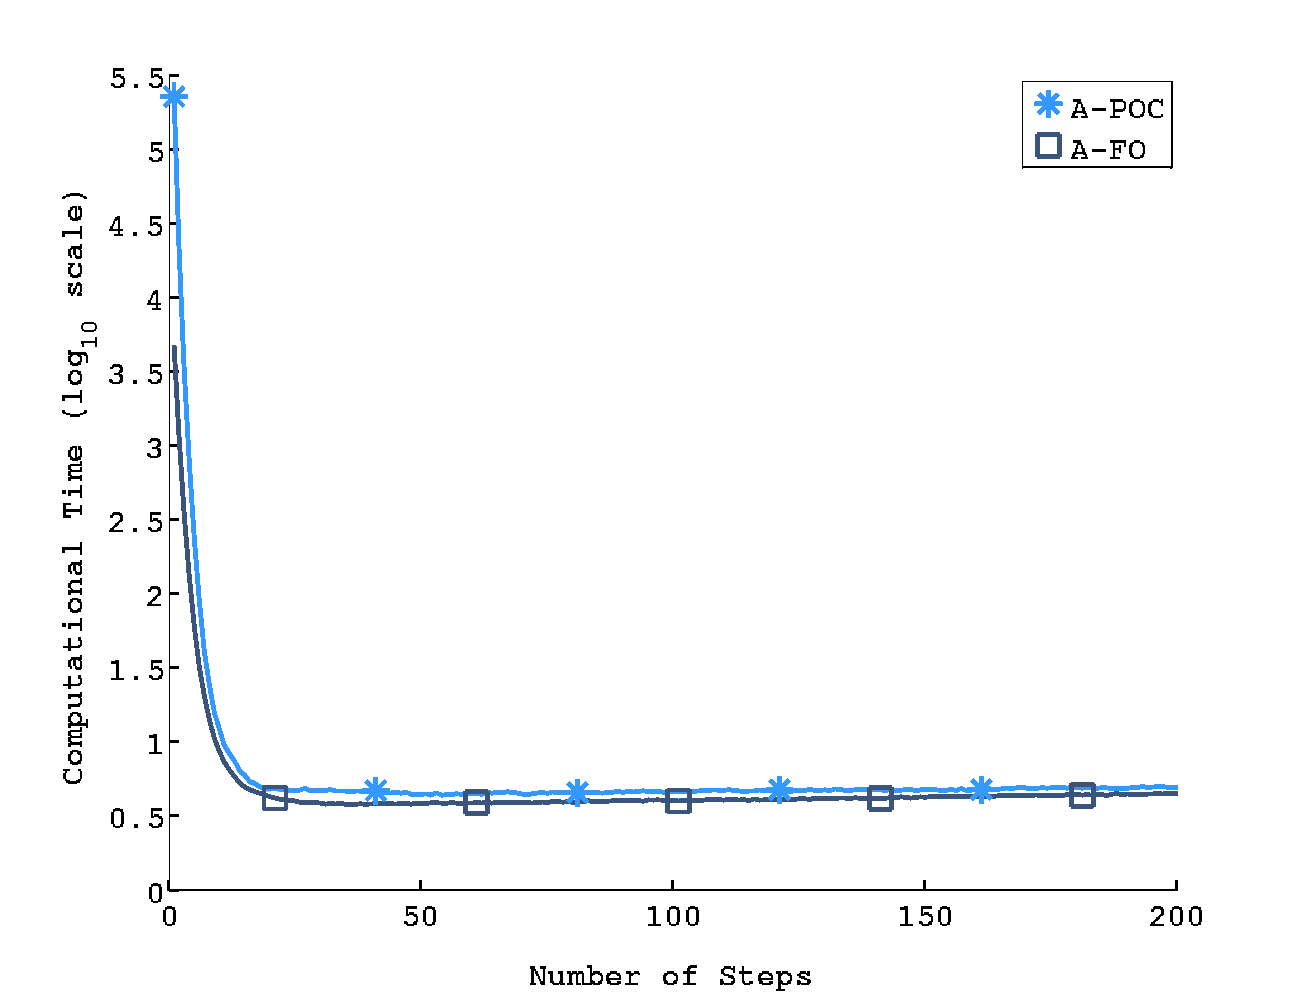
\includegraphics[trim=1.5cm 0cm 2.7cm 1.8cm, clip=true,width=\columnwidth]{plots/with_noise/computationalTime.png}
%     \caption{With 20\% noise}
%     \label{subfig:comptimewithnoise}
%   \end{subfigure}
%   \caption{Comparison of the computational time per step (log scale) between different ad hoc agent. The more hypotheses the more initial computational time. After 20 steps, most hypotheses are discarded and the updates become faster.}
%   \label{fig:comptime}
% \end{figure}

% \todo{Our results show that the default teams we built are not optimal. Indeed an ad hoc agent, that is not always taking the action the agent it replaces would have chosen, can on average achieve similar performance. It the default team where optimal, we would expect the performance profile to have the same slope but a small ``delay'' -- loosing some important steps in the beginning. A more advanced planning method for the ad hoc agent could even improve the performance of all team, as described in \cite{barrett2011empirical}}
